\documentclass{article}

\usepackage[tmargin=0.5in,bmargin=0.25in]{geometry}
\usepackage{amsmath, amssymb, amsthm}
\usepackage{enumitem}
\usepackage{graphicx}
\usepackage{listings}

\graphicspath{.}

\title{\vspace{-5ex}M/CS 375 Project 1}
\author{Isaac Boaz}

\begin{document}
\maketitle

\begin{enumerate}
    \item Taylor Polynomials
          \begin{enumerate}[label=(\alph*)]
                \item Degree 5 Taylor Polynomial for \(f(x) = cos x\) where \(x_0 = 0\).
                      \begin{align*}
                          P_5(x) &= \sum_{k=0}^5 \frac{f^{(k)}(x_0)}{k!}(x-x_0)^k \\
                          &= cos(0) - sin(0)x - \frac{cos(0)x^2}{2} + \frac{sin(0)x^3}{6} - \frac{cos(0)x^4}{24} + \frac{sin(0)x^5}{120} \\
                          &= 1 - \frac{x^2}{2!} + \frac{x^4}{4!} \\
                      \end{align*}
                \item Worst-case error for \(x\) in \(\lbrack -\frac{\pi}{4}, \frac{\pi}{4}\rbrack\)
                      \begin{align*}
                        E_{5+1} &= \frac{1}{6!}f^{(6)}(c)(x)^6 \\
                        &= \frac{1}{720} -cos(c)(x)^6 \\
                        &= \frac{\frac{\pi}{4}^6}{720}cos(c) \\
                        &< \frac{0.2397}{720} < 3 \times 10^{-4}
                      \end{align*}
                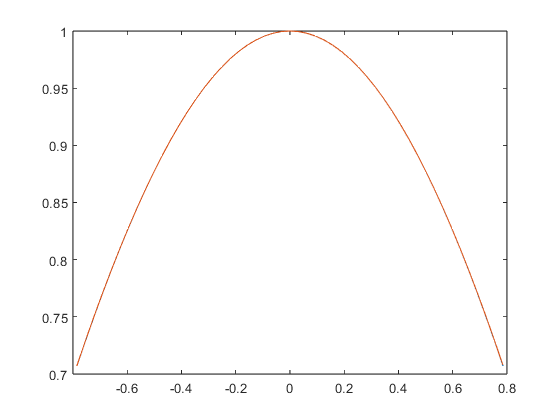
\includegraphics[scale=0.50]{cosgraph.png}
                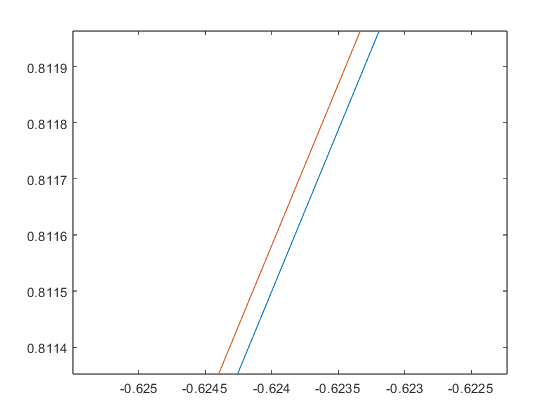
\includegraphics[scale=0.5]{cosgraph_zoomed.png}
          \end{enumerate}
    \item MatLab 
    \lstset{language=MatLab,basicstyle=\small\ttfamily}
          \begin{enumerate}[label=(\alph*)]
            \item \(f(x) = 230x^4 + 18x^3 + 9x^2 - 221x - 9;\ [0, 1]\)
\begin{lstlisting}N: 1.893157e+01
Iterating 19 times
 k   A          B          c           f(c)
 0:  0.0000000  1.0000000  0.5000000 -100.6250000
 1:  0.5000000  1.0000000  0.7500000 -89.3203125
 2:  0.7500000  1.0000000  0.8750000 -48.6040039
 3:  0.8750000  1.0000000  0.9375000 -15.7762756
 4:  0.9375000  1.0000000  0.9687500   4.2870235
 5:  0.9375000  0.9687500  0.9531250  -6.0654713
 6:  0.9531250  0.9687500  0.9609375  -0.9707179
 7:  0.9609375  0.9687500  0.9648438   1.6376179
 8:  0.9609375  0.9648438  0.9628906   0.3283365
 9:  0.9609375  0.9628906  0.9619141  -0.3224666
10:  0.9619141  0.9628906  0.9624023   0.0026157
11:  0.9619141  0.9624023  0.9621582  -0.1600052
12:  0.9621582  0.9624023  0.9622803  -0.0787147
13:  0.9622803  0.9624023  0.9623413  -0.0380545
14:  0.9623413  0.9624023  0.9623718  -0.0177207
15:  0.9623718  0.9624023  0.9623871  -0.0075528
16:  0.9623871  0.9624023  0.9623947  -0.0024686
17:  0.9623947  0.9624023  0.9623985   0.0000735
18:  0.9623947  0.9623985  0.9623966  -0.0011976
19:  0.9623966  0.9623985  0.9623976  -0.0005620

ans =

   0.962397575378418
            \end{lstlisting}
        \item \(f(x) = 1 + ln(1+x^2);\ [0, 1]\)
        \begin{lstlisting}
1.000000 and 1.693147 must be opposite signs
        \end{lstlisting}
        \item \(f(x) = e^x + 2^{-x} + 2cosx - 6;\ [1, 2]\)
        \begin{lstlisting}
Iterating 19 times
k   A          B          c           f(c)
0:  1.0000000  2.0000000  1.5000000  -1.0232831
1:  1.5000000  2.0000000  1.7500000  -0.3045877
2:  1.7500000  2.0000000  1.8750000   0.1943790
3:  1.7500000  1.8750000  1.8125000  -0.0682744
4:  1.8125000  1.8750000  1.8437500   0.0596374
5:  1.8125000  1.8437500  1.8281250  -0.0051567
6:  1.8281250  1.8437500  1.8359375   0.0270289
7:  1.8281250  1.8359375  1.8320312   0.0108835
8:  1.8281250  1.8320312  1.8300781   0.0028502
9:  1.8281250  1.8300781  1.8291016  -0.0011565
10:  1.8291016  1.8300781  1.8295898   0.0008460
11:  1.8291016  1.8295898  1.8293457  -0.0001554
12:  1.8293457  1.8295898  1.8294678   0.0003453
13:  1.8293457  1.8294678  1.8294067   0.0000949
14:  1.8293457  1.8294067  1.8293762  -0.0000303
15:  1.8293762  1.8294067  1.8293915   0.0000323
16:  1.8293762  1.8293915  1.8293839   0.0000010
17:  1.8293762  1.8293839  1.8293800  -0.0000146
18:  1.8293800  1.8293839  1.8293819  -0.0000068
19:  1.8293819  1.8293839  1.8293829  -0.0000029

ans =

    1.829382896423340
        \end{lstlisting}
    \end{enumerate}
    \item Interest Rate
    \begin{lstlisting}
Iterating 12 times
k   A          B          c           f(c)
0:  0.0000000  0.0500000  0.0250000 -535.4359178
1:  0.0250000  0.0500000  0.0375000 436.7535239
2:  0.0250000  0.0375000  0.0312500 -72.5564497
3:  0.0312500  0.0375000  0.0343750 176.0219417
4:  0.0312500  0.0343750  0.0328125  50.2486600
5:  0.0312500  0.0328125  0.0320312 -11.5206196
6:  0.0320312  0.0328125  0.0324219  19.2718057
7:  0.0320312  0.0324219  0.0322266   3.8526063
8:  0.0320312  0.0322266  0.0321289  -3.8397450
9:  0.0321289  0.0322266  0.0321777   0.0049950
10:  0.0321289  0.0321777  0.0321533  -1.9177338
11:  0.0321533  0.0321777  0.0321655  -0.9564591
12:  0.0321655  0.0321777  0.0321716  -0.4757545

ans =

    0.032171630859375
    \end{lstlisting}
\end{enumerate}

\end{document}